\newcommand{\import}[1]{\input{présentation/#1}}
%–––––––––––––––––––––––––––––––––––––––––––––––––––––––––––––––––––––––––––––––
\import{settings}
\import{plan}
%–––––––––––––––––––––––––––––––––––––––––––––––––––––––––––––––––––––––––––––––
\import{introduction}
\import{principles}
\import{examples}
\import{critics}
\import{conclusion}
%–––––––––––––––––––––––––––––––––––––––––––––––––––––––––––––––––––––––––––––––
\section{Questions}
%⋅⋅⋅⋅⋅⋅⋅⋅⋅⋅⋅⋅⋅⋅⋅⋅⋅⋅⋅⋅⋅⋅⋅⋅⋅⋅⋅⋅⋅⋅⋅⋅⋅⋅⋅⋅⋅⋅⋅⋅⋅⋅⋅⋅⋅⋅⋅⋅⋅⋅⋅⋅⋅⋅⋅⋅⋅⋅⋅⋅⋅⋅⋅⋅⋅⋅⋅⋅⋅⋅⋅⋅⋅⋅⋅⋅⋅⋅⋅
\begin{frame}{\bititle\\Questions}
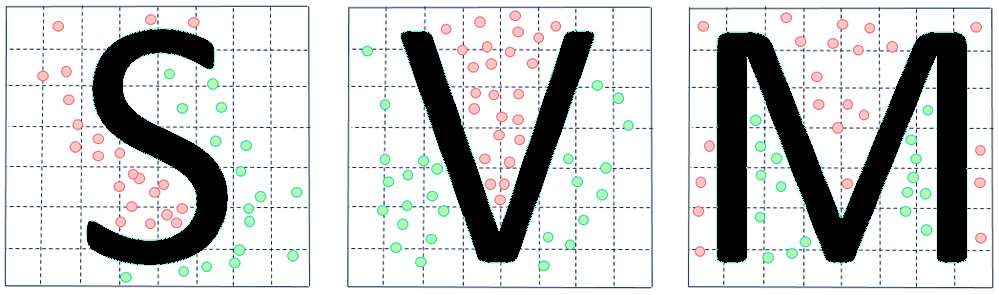
\includegraphics[width=\textwidth]{images/svm}
\end{frame}
%–––––––––––––––––––––––––––––––––––––––––––––––––––––––––––––––––––––––––––––––
\end{document}
